\documentclass{article}

\usepackage{amsmath} % For align*, etc.
\usepackage{circuitikz} % For circuit diagrams
\usepackage{bookmark} % For links
\usepackage{float} % For the [H] option on figures
\usepackage{graphicx} % For images
\usepackage{tikz} % For diagrams
\usepackage{siunitx} % For units

% Set up packages
\graphicspath{{./images/}}
\hypersetup{
  colorlinks=true,
  linkcolor=blue,
  urlcolor=blue
}

% Declare custom commands
\DeclareMathOperator{\rank}{rank}
\renewcommand{\vec}[1]{\boldsymbol{\mathbf{#1}}}
\newcommand{\dvec}[1]{\dot{\vec{#1}}}

\title{How I Made a Self-Balancing Inverted Pendulum}
\author{Chris Doble}
\date{February 2024}

\begin{document}

\maketitle

\tableofcontents

\section{Introduction}

I recently built a self-balancing inverted pendulum. You can watch a video of it \href{https://www.youtube.com/watch?v=-cd6RuVWI30}{here}. If you've ever tried to keep something like a broom or a stick upright on your hand you'll know it can be quite tricky! Gravity's constantly pulling it down, so if it’s not perfectly vertical it’ll start to fall. The same thing happens to the pendulum but it's connected to a cart which is programmed to move left and right in a way that keeps the pendulum upright.

In this document I’ll explain how I built it. We'll start by deriving the system's equations of motion, then we'll linearise them so we can make use of some tools from linear control theory. Those tools will help us determine if the system is stable and how to control it. We'll talk about the physical construction of the system and how that integrates with the mathematical model. Finally we'll talk about the code that controls it.

\section{Equations of Motion}

If we want to control this system we need to know how it behaves, so let’s derive its equations of motion. First we need to define our coordinate system and variables in a diagram:

\begin{figure}[H]
  \centering
  \begin{tikzpicture}
    % x
    \draw (-2, 0.3) -- (-2, 0.7);
    \draw[dashed] (-2, 0.5) -- node[above] {$x$} (0, 0.5);

    % Cart
    \draw (0, 0) rectangle node {$m_1$} (2, 1);

    % Pendulum
    \draw (1, 1) -- (0.5, 3);
    \draw[dashed] (1, 1) -- (1, 3);
    \draw (0.37, 3.4) node {$m_2$} circle (0.4cm);

    % l
    \node at (0.5, 1.8) {$l$};

    % Theta
    \draw (1, 2.8) arc (90:117:1);
    \node at (0.8, 2.5) {$\theta$};

    % Axes
    \draw[->] (3, 0.5) -- (4, 0.5) node[right] {$x$};
    \draw[->] (3, 0.5) -- (3, 1.5) node[above] {$y$};
  \end{tikzpicture}
\end{figure}

We have a cart of mass $m_1$. Its $x$ position is measured from some origin point and it can only move along the $x$-axis. The cart is connected to a simple pendulum of length $l$ and mass $m_2$ and it's at an angle $\theta$ from vertical.

With that out of the way, now we can calculate the Lagrangian of the system. The Lagrangian is defined as the difference between the system's kinetic and potential energies \[\mathcal{L} = T - U.\]

Starting with the cart, its kinetic energy is \[T_\text{cart} = \frac{1}{2} m_1 v^2\] but because it can only move along the $x$-axis its velocity has no $y$ component and this is equivalent to \[T_\text{cart} = \frac{1}{2} m_1 \dot{x}^2\] where $\dot{x}$ is the derivative of $x$ with respect to time, i.e. the cart's $x$ velocity. As for the cart's potential energy, it can't move up or down so its gravitational potential energy can't change and there's no springs or anything involved so we might as well set it to \[U_\text{cart} = 0.\]

Next, the pendulum. Because it's joined to the cart its $x$ coordinate changes as the cart moves, and both of its coordinates change as it rotates. That being the case, its coordinates are \begin{align*}
  X & = x - l \sin \theta \\
  Y & = l \cos \theta.
\end{align*} Differentiating them with respect to time gives the $x$ and $y$ components of the pendulum's velocity \begin{align*}
  \dot{X} & = \dot{x} - l \dot{\theta} \cos \theta \\
  \dot{Y} & = -l \dot{\theta} \sin \theta.
\end{align*} Using the Pythagorean theorem we can combine these to find the squared magnitude of its velocity \begin{align*}
  V^2 & = \dot{X}^2 + \dot{Y}^2                                                      \\
      & = (\dot{x} - l \dot{\theta} \cos \theta)^2 + (-l \dot{\theta} \sin \theta)^2 \\
      & = \dot{x}^2 - 2 l \dot{\theta} \dot{x} \cos \theta + l^2 \dot{\theta}^2
\end{align*}
and we can use this to find its kinetic energy \begin{align*}
  T_\text{pendulum} & = \frac{1}{2} m_2 V^2                                                                      \\
                    & = \frac{1}{2} m_2 (\dot{x}^2 - 2 l \dot{\theta} \dot{x} \cos \theta + l^2 \dot{\theta}^2).
\end{align*} Unlike the cart, the pendulum's potential energy can change — when it rotates it moves up and down so its gravitational potential energy changes. If we say its potential energy is $0$ when it's horizontal ($\theta = \pi / 2$), then we can define its potential energy to be \begin{align*}
  U_\text{pendulum} & = m_2 g y             \\
                    & = m_2 g l \cos \theta
\end{align*} where $g$ is acceleration due to gravity.

Combining all of those energies and rearranging gives us our Lagrangian \begin{align*}
  \mathcal{L} & = T - U                                                                                                                                     \\
              & = T_\text{cart} + T_\text{pendulum} - U_\text{cart} - U_\text{pendulum}                                                                     \\
              & = \frac{1}{2} m_1 \dot{x}^2 + \frac{1}{2} m_2 (\dot{x}^2 - 2 l \dot{\theta} \dot{x} \cos \theta + l^2 \dot{\theta}^2) - m_2 g l \cos \theta \\
              & = \frac{1}{2} (m_1 + m_2) \dot{x}^2 + \frac{1}{2} m_2 (l^2 \dot{\theta}^2 - 2 l \dot{\theta} \dot{x} \cos \theta) - m_2 g l \cos \theta.
\end{align*}

Now that we have it we can apply the Euler-Lagrange equation to each of the system's two coordinates $\theta$ and $x$. For $\theta$ we get \begin{align*}
  0 & = \frac{\partial \mathcal{L}}{\partial \theta} - \frac{d}{d t} \frac{\partial \mathcal{L}}{\partial \dot{\theta}}                                            \\
    & = m_2 l \dot{\theta} \dot{x} \sin \theta + m_2 g l \sin \theta - \frac{d}{d t} (m_2 l^2 \dot{\theta} - m_2 l \dot{x} \cos \theta)                            \\
    & = m_2 l \dot{\theta} \dot{x} \sin \theta + m_2 g l \sin \theta - m_2 l^2 \ddot{\theta} + m_2 l \ddot{x} \cos \theta - m_2 l \dot{\theta} \dot{x} \sin \theta \\
    & = g \sin \theta - l \ddot{\theta} + \ddot{x} \cos \theta                                                                                                     \\
\end{align*} and for $x$ we get \begin{align*}
  0 & = \frac{\partial \mathcal{L}}{\partial x} - \frac{d}{d t} \frac{\partial L}{\partial \dot{x}} \\
    & = -\frac{d}{d t} [(m_1 + m_2) \dot{x} - m_2 l \dot{\theta} \cos \theta]                       \\
    & = -(m_1 + m_2) \ddot{x} + m_2 l \ddot{\theta} \cos \theta - m_2 l \dot{\theta}^2 \sin \theta.
\end{align*} Rearranging these two equations and solving for $\ddot{\theta}$ and $\ddot{x}$ gives us our equations of motion \begin{align*}
  \ddot{\theta} & = \frac{(m_1 + m_2) g \sin \theta - m_2 l \dot{\theta}^2 \cos \theta \sin \theta}{l (m_1 + m_2) - m_2 l \cos^2 \theta} \\
  \ddot{x}      & = \frac{m_2 g \sin 2 \theta - 2 m_2 l \dot{\theta}^2 \sin \theta}{2 m_1 + m_2 - m_2 \cos 2 \theta}.
\end{align*}

Now that we have them how do we know they're correct? One way would be to solve them for $\theta$ and $x$ and see if their predictions are reasonable. I certainly don't know how to solve them analytically, but we can solve them numerically. \href{https://github.com/chrisdoble/self-balancing-inverted-pendulum/blob/master/notebooks/uncontrolled.nb}{Here} is a Mathematica notebook that does just that. First it defines some constants like gravity, the length of the pendulum, etc. followed by the initial conditions for the simulation. It solves the equations of motion numerically and generates a plot of the solutions. The following shows a pendulum being released from $\ang{30}$.

\begin{figure}[H]
  \centering
  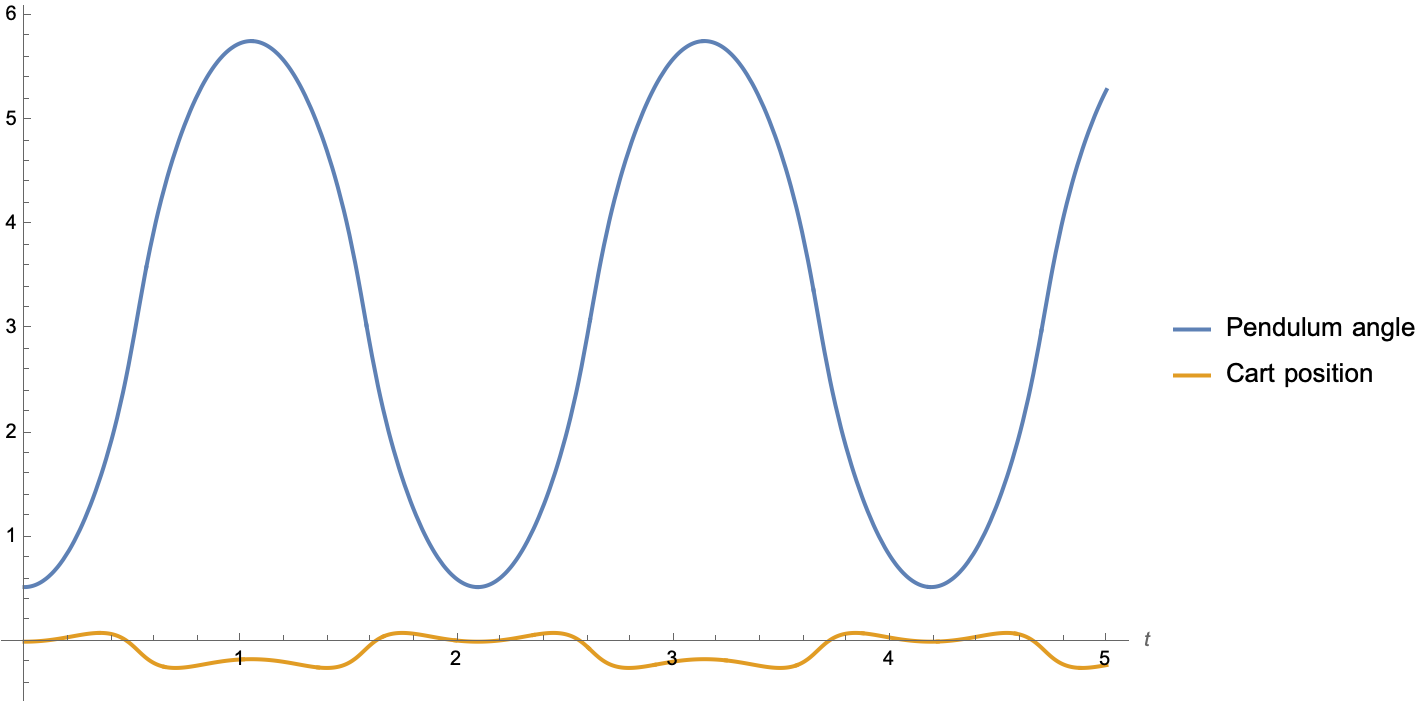
\includegraphics[width=\textwidth]{uncontrolled}
\end{figure}

The pendulum swings back and forth as we expect, but interestingly it also causes the cart to move. The notebook also generates an animation which you can see \href{https://github.com/chrisdoble/self-balancing-inverted-pendulum/blob/master/post/images/uncontrolled.gif}{here}.

\section{Linearisation}

These equations look good, but they're quite complicated so it might be difficult to analyse the stability of the system and determine how to control it. Can we simplify them at all? One approach is to linearise them.

Linearising a function means finding a linear approximation of it at a particular point. For example, if we graph a function $y = f(x)$ and we want to linearise it at $x = 1$, we evaluate it at the point to find its $y$ coordinate, and we evaluate its derivative at the point to find its slope. Using this information we can plot a new function that passes through the point and extends the slope in both directions. It's a line. Near the point the line does a pretty good job of approximating the function. As you move away it doesn't do as good of a job, but if you only care about the region around the point that's fine.

\begin{figure}[H]
  \centering
  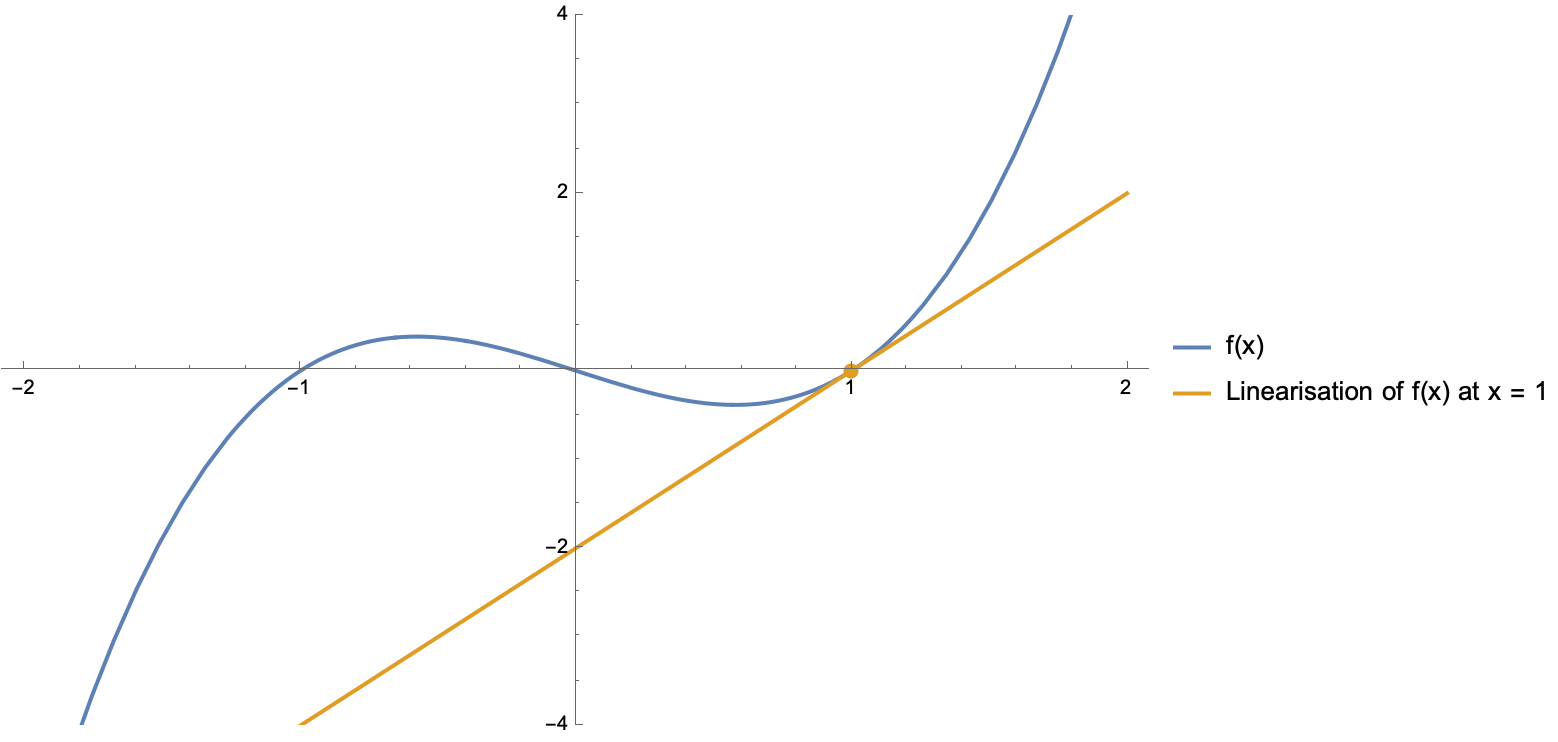
\includegraphics[width=\textwidth]{linearisation}
\end{figure}

In the case of the pendulum, our goal is to keep the cart in the middle of the track, the pendulum upright, and neither the cart nor the pendulum moving. In other words, we want all four variables $\theta$, $\dot{\theta}$, $x$, and $\dot{x}$ to be $0$. The further they are from $0$ the less likely it is we'll be able to recover and we might have to accept that the pendulum's going to fall over or hit the end of the track. If they're always going to be near $0$ then it sounds like we can tolerate the approximation error and linearisation might work for us!

So how do we linearise our equations of motion? First, let's combine them into one vector-valued function \[\begin{bmatrix}
    \ddot{\theta} \\
    \ddot{x}
  \end{bmatrix} = \vec{f}(\theta, \dot{\theta}) = \begin{bmatrix}
    \frac{(m_1 + m_2) g \sin \theta - m_2 l \dot{\theta}^2 \cos \theta \sin \theta}{l (m_1 + m_2) - m_2 l \cos^2 \theta} \\
    \frac{m_2 \sin 2 \theta - 2 m_2 l \dot{\theta}^2 \sin \theta}{2 m_1 + m_2 - m_2 \cos 2 \theta}
\end{bmatrix}.\] Let's also define the state vector $\vec{x}$ to be a column matrix describing the state of the system \[\vec{x} = \begin{bmatrix} \theta \\ \dot{\theta} \\ x \\ \dot{x} \end{bmatrix}.\] With this definition we can change our function to accept the state vector $\vec{x}$ \[\begin{bmatrix}
    \ddot{\theta} \\
    \ddot{x}
  \end{bmatrix} = \vec{f}(\vec{x}) = \begin{bmatrix}
    \frac{(m_1 + m_2) g \sin \theta - m_2 l \dot{\theta}^2 \cos \theta \sin \theta}{l (m_1 + m_2) - m_2 l \cos^2 \theta} \\
    \frac{m_2 \sin 2 \theta - 2 m_2 l \dot{\theta}^2 \sin \theta}{2 m_1 + m_2 - m_2 \cos 2 \theta}
  \end{bmatrix}.\] If we include $\dot{\theta}$ and $\dot{x}$ in the output you can see that the function now returns the derivative of $\vec{x}$ \begin{align*}
  \begin{bmatrix}
    \dot{\theta}  \\
    \ddot{\theta} \\
    \dot{x}       \\
    \ddot{x}
  \end{bmatrix} & = \vec{f}(\vec{x}) = \begin{bmatrix}
                                         \dot{\theta}                                                                                                         \\
                                         \frac{(m_1 + m_2) g \sin \theta - m_2 l \dot{\theta}^2 \cos \theta \sin \theta}{l (m_1 + m_2) - m_2 l \cos^2 \theta} \\
                                         \dot{x}                                                                                                              \\
                                         \frac{m_2 \sin 2 \theta - 2 m_2 l \dot{\theta}^2 \sin \theta}{2 m_1 + m_2 - m_2 \cos 2 \theta}
                                       \end{bmatrix}    \\
  \dvec{x}         & = \vec{f}(\vec{x}) = \begin{bmatrix}
                                            \dot{\theta}                                                                                                         \\
                                            \frac{(m_1 + m_2) g \sin \theta - m_2 l \dot{\theta}^2 \cos \theta \sin \theta}{l (m_1 + m_2) - m_2 l \cos^2 \theta} \\
                                            \dot{x}                                                                                                              \\
                                            \frac{m_2 \sin 2 \theta - 2 m_2 l \dot{\theta}^2 \sin \theta}{2 m_1 + m_2 - m_2 \cos 2 \theta}
                                          \end{bmatrix}.
\end{align*}

The general equation to linearise a vector-valued function like this at a particular point $\vec{p}$ is \[\vec{f}(\vec{x}) \approx f(\vec{p}) + D \vec{f}|_{\vec{p}} (\vec{x} - \vec{p}).\] As mentioned before we want to linearise our function at the point where all the elements of $\vec{x}$ are $0$. That means $\vec{p}$ is the zero vector and the equation becomes \[\vec{f}(\vec{x}) \approx f(\vec{0}) + D \vec{f}|_{\vec{0}} (\vec{x} - \vec{0}).\] Looking at the elements within $\vec{f}(\vec{x})$ you can see that at this point $\dot{\theta} = 0$ so the first element is $0$. $\sin \theta = 0$ so the second element is $0$. $\dot{x} = 0$ so the third element is $0$. Finally, $\sin \theta = 0$ and $\sin 2 \theta = 0$ so the fourth element is $0$. So $\vec{f}(\vec{x})$ evaluated at the point $\vec{p} = \vec{0}$ is also the zero vector and we can remove it from our linearised function \[\vec{f}(\vec{x}) \approx D \vec{f}|_{\vec{0}} \vec{x}.\]

The remaining term is the Jacobian matrix of our function evaluated at the point $\vec{p} = \vec{0}$. It plays the same role the derivative did in the previous two-dimensional example — when you multiply it by a displacement vector $\vec{x}$ it tells you how much each component of the function differs from the point at which it was linearised. It's like extending the slope in each dimension. If we actually evaluate it we get a matrix that we'll call $\vec{A}$ and the final linearised version of our function is \[\dvec{x} = \vec{A} \vec{x} = \begin{bmatrix}
    0                           & 1 & 0 & 0 \\
    \frac{g (m_1 + m_2)}{l m_1} & 0 & 0 & 0 \\
    0                           & 0 & 0 & 1 \\
    \frac{g m_2}{m_1}           & 0 & 0 & 0
  \end{bmatrix} \vec{x}.\]

I've intentionally skimmed over some details in this section to keep things short. If you'd like to learn more about linearising nonlinear systems and when it's actually valid to do that, these two videos from Steve Brunton are great: \href{https://www.youtube.com/watch?v=RCWkzzLgwf0}{Linearizing Nonlinear Differential Equations Near a Fixed Point}, and \href{https://www.youtube.com/watch?v=vRaUSnB7qNw}{The Hartman-Grobman Theorem, Structural Stability of Linearization, and Stable/Unstable Manifolds}.

\section{Stability}

Now that we have a linearised version of our equations of motion we can apply some tools from linear control theory. One of those tools is stability analysis. This tells us that if any of the eigenvalues of our $\vec{A}$ matrix have a positive real component, the system is unstable. Our four eigenvalues are \[0, \ 0, \ -\sqrt{\frac{g (m_1 + m_2)}{l m_1}}, \text{ and } \sqrt{\frac{g (m_1 + m_2)}{l m_1}}.\] All of the values under that radical are positive, so the second two eigenvalues are real and the last eigenvalue is positive which tells us what we already know: the pendulum's going to fall over.

\section{Control}

I mentioned earlier that the cart moves left and right to keep the pendulum upright. A more formal of saying that is: we can say we apply a force $F$ on the cart in the $x$ direction. We can recalculate our equations of motion to include this force, the only difference is we apply d'Alembert's principle to the Euler-Lagrange equation for the $x$ coordinate and equate it to $F$. This results in the following updated equations of motion where I've hidden some terms so we can focus on the coefficients of $F$ \begin{align*}
  \ddot{\theta} & = f(\theta, \dot{\theta}) + \frac{\cos \theta}{l (m_1 + m_2) - l m_2 \cos^2 \theta} F \\
  \ddot{x}      & = g(\theta, \dot{\theta}) + \frac{2}{2 m_1 + m_2 - m_2 \cos 2 \theta} F.
\end{align*} Again, our goal is for $\theta$ to be close to $0$ so we can use the small angle approximation where $\cos \theta \approx 1$. That simplifies these equations to \begin{align*}
  \ddot{\theta} & = f(\theta, \dot{\theta}) + \frac{1}{l m_1} F \\
  \ddot{x}      & = g(\theta, \dot{\theta}) + \frac{1}{m_1} F.
\end{align*} If we use the coefficients of $F$ to create a new matrix $\vec{B}$ and substitute this into our linearised equations of motion we get \begin{align*}
\dvec{x} &= \vec{A} \vec{x} + \vec{B} F \\
&= \begin{bmatrix}
    0                           & 1 & 0 & 0 \\
    \frac{g (m_1 + m_2)}{l m_1} & 0 & 0 & 0 \\
    0                           & 0 & 0 & 1 \\
    \frac{g m_2}{m_1}           & 0 & 0 & 0
  \end{bmatrix} \vec{x} + \begin{bmatrix}
    0               \\
    \frac{1}{l m_1} \\
    0               \\
    \frac{1}{m_1}
\end{bmatrix} F.
\end{align*}

Another useful tool from control theory is the concept of controllability. A system is said to be controllable if it's possible to move it into any state you want using only its inputs. In our case, the only input is $F$ — is that enough to control the system? It is if the rank of the controllability matrix equals the dimension of the state space \begin{align*}
\rank(\vec{C}) &= \rank(\begin{bmatrix}
\vec{B} & \vec{A} \vec{B} & \vec{A}^2 \vec{B} & \cdots & \vec{A}^{n - 1} \vec{B}
\end{bmatrix}) \\
&= n.
\end{align*} If we perform this calculation using our $\vec{A}$ and $\vec{B}$ matrices we get the value $4$. This is the dimension of our state vector which means we are able to control the system using only the force $F$.

Now we have a way to control the system, but how do we choose $F$? We want it to be a function of the state of the system — for example, if the pendulum is close to vertical we want to apply a small force but if it's far from vertical we want to apply a larger force. This suggests we could define it as a row matrix $\vec{K}$ times the state vector $\vec{x}$ \[F = \vec{K} \vec{x}.\] Conventionally this is written with a minus sign \[F = -\vec{K} \vec{x}.\]

If we substitute this into our linearised equation of motion we get \begin{align*}
  \dvec{x} & = \vec{A} \vec{x} - \vec{B} \vec{K} \vec{x} \\
           & = (\vec{A} - \vec{B} \vec{K}) \vec{x}.
\end{align*} This looks very similar to the original equation except $\vec{A}$ has been replaced by $\vec{A} - \vec{B} \vec{K}$. If we can choose $\vec{K}$ in such a way that the eigenvalues of $\vec{A} - \vec{B} \vec{K}$ don't have positive real components, the system will be stable.

So how do we choose $\vec{K}$? One approach is to use the Linear Quadratic Regulator algorithm. I don't completely understand how this works, but thankfully there's a Mathematica function that does. It accepts our $\vec{A}$ and $\vec{B}$ matrices plus two additional matrices that define how much it ``costs'' to apply a force to the cart and for each variable to differ from $0$. For example, if we don't want to use much electricity running the motor we could set the force cost high and the resulting $\vec{K}$ matrix would try to minimise its use. Or if we don't want the cart to move far from the centre of the track we could set the $x$ cost high and the matrix would try to keep it near $0$, possibly at the expense of another variable like the pendulum angle.

\href{https://github.com/chrisdoble/self-balancing-inverted-pendulum/blob/master/notebooks/controlled.nb}{Here} is a Mathematica notebook that calculates the $\vec{K}$ matrix and generates a plot of a pendulum controlled by it. The following shows a pendulum being released from $\ang{30}$ with all costs set to $1$.

\begin{figure}[H]
  \centering
  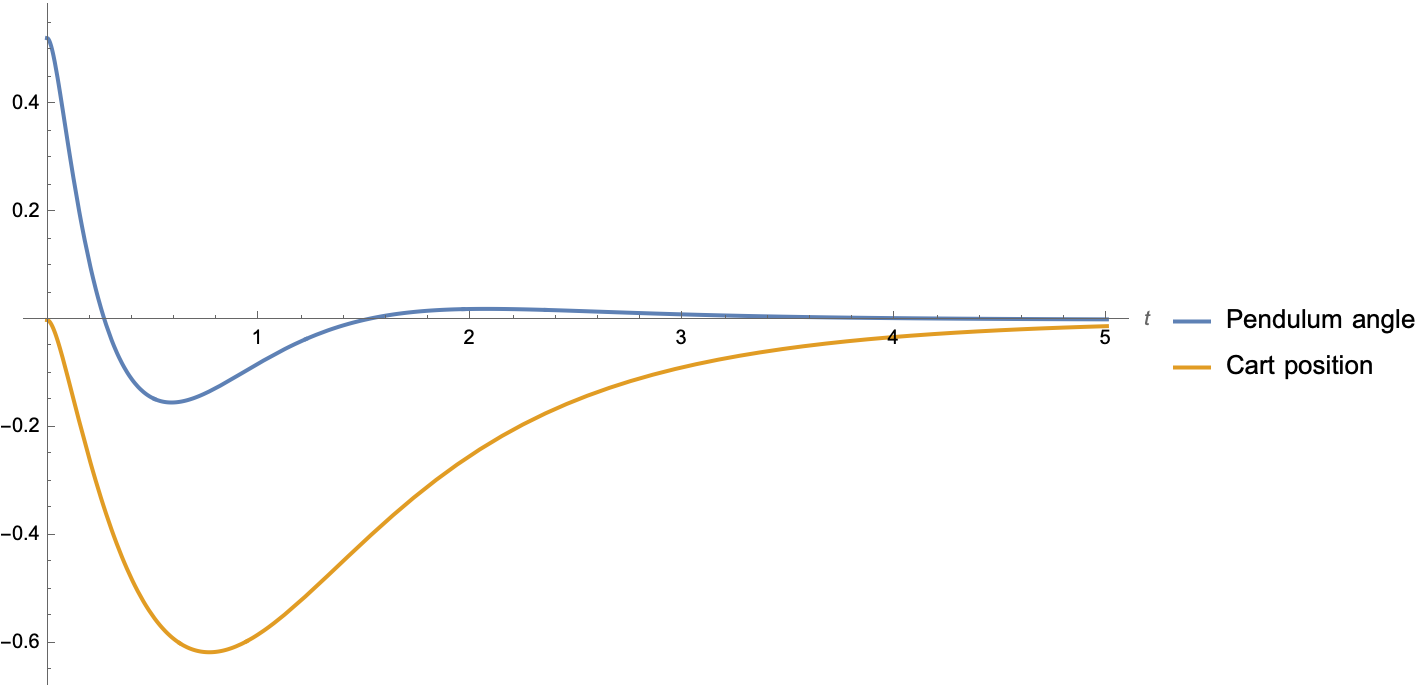
\includegraphics[width=\textwidth]{controlled}
\end{figure}

The cart quickly moves to the left to prevent the pendulum from falling, continues moving until the pendulum is slightly angled to the right, then slowly moves to the right until the cart is in the middle of the track and the pendulum is vertical.

\section{Building}

That's enough math for now. Let's talk about how I built it!

This is a model of the system that I designed in Fusion 360. At the core are two steel rods that the cart slides along on linear bearings. The cart itself and the two ends are 3D printed in PLA. On the bottom of the cart are two extensions that the timing belt connects to, but it's not visible in this model. The timing belt comes from one side of the cart, over the ilder pulley, all the way over to the timing pulley, and back to the other side of the cart. This means that when the timing pulley rotates, the cart moves.

The timing pulley is on an axle that's connected to an incremental rotary encoder so we can measure the position of the cart. On the other side of the axle is a 3D printed 5:1 gear train that's connected to a DC motor. I had to add the gear train because I bought a 24V motor which ended up being overkill for this project and I needed a way to reduce the RPM. On top of the housing is a limit switch which is primarily used to zero the cart position on startup, but it's also used to kill the motor if the cart gets too close to the end.

The pendulum itself is a long steel rod connected to a shorter steel rod with a 90° clamp. The shorter rod runs through some bearings and to another incremental rotary encoder that lets us measure the angle of the pendulum.

The system is all controlled by an Arduino Uno, the motor is controlled by a motor driver which is connected to a 24V power supply, and everything is connected via a breadboard.

After printing and assembling everything this is what it looks like. You can see that there are some long wires connected to the cart so it can move around.

\section{Motor Control}

Great! We have our control algorithm and we've built the physical system, but there's still one missing piece. The control algorithm tells us the force $F$ to apply to the cart, but the Arduino controls the cart via a motor, and it controls the motor via a voltage. How do we convert a force into a voltage? We'll need an equation for that.

\begin{figure}[H]
  \centering
  \begin{circuitikz}[american voltages]
    \draw (0, 0) to [V, invert, l=$V_\text{in}$] (0, 2)
    to [resistor, l=$R$] (3, 2)
    to [inductor, l=$L$] (5, 2)
    to [V, l=$V_\text{motor}$] (5, 0)
    to (0, 0);
  \end{circuitikz}
\end{figure}

We can model the electrical properties of a DC motor using this simple circuit. $V_\text{in}$ is the voltage applied to the motor, $R$ is the resistance of its windings, $L$ is the inductance of its windings, and $V_\text{motor}$ is the back emf generated as the motor is spinning. Applying Kirchoff's voltage law to this circuit gives \[V_\text{in} - I R - \frac{d I}{d t} L - V_\text{motor} = 0.\] If we assume the back emf is proportional to the motor's angular velocity $\omega$ the final term becomes $a_1 \omega$ where $a_1$ is a proportionality constant \[V_\text{in} - I R - \frac{d I}{d t} L - a_1 \omega = 0.\]

We can model the mechanical properties of a DC motor by treating it as a rotating cylinder. It experiences a torque from the motor $\tau_m$ and a resistive torque $\tau_r$ from back emf, friction, etc. This gives an equation of motion \[\tau_m - \tau_r = J \dot{\omega}\] where $J$ is the cylinder's moment of inertia. If we assume the torque from the motor is proportional to the current flowing through it this becomes \[a_2 I - \tau_r = J \dot{\omega}\] and if we further assume that the resistive torque is proportional to the cylinder's angular velocity this becomes \[a_2 I - a_3 \omega = J \dot{\omega}.\]

We can solve this equation of motion for $I$ and take the derivative of that expression to find one for $\frac{d I}{d t}$. If we substitute these into the electrical equation and collect constants we get \[b_1 \ddot{\omega} + b_2 \dot{\omega} + b_3 \omega + V_\text{in} = 0\] which has the general solution \[\omega = c_1 V_\text{in} + c_2 e^{c_3 t} + c_4 e^{c_5 t}.\]

Taking a step back, what does this equation represent? It tells us how the motor's angular velocity changes over time if we apply a constant voltage $V_\text{in}$. Can we use our intuition about how the motor behaves to give us any clues about these constants? First of all, we probably don't need two exponential terms, so let's assume $c_4$ is $0$ \[\omega = c_1 V_\text{in} + c_2 e^{c_3 t}.\] Next, the motor's angular velocity is $0$ at $t = 0$ so $c_2 = -c_1 V_\text{in}$ \[\omega = c_1 V_\text{in} (1 - e^{c_3 t}).\] We also know that if we apply a constant voltage the motor's angular velocity will increase quite quickly but then resistive forces cause it to stabilise around a steady state value. If that's the case $c_3$ must be negative, otherwise the angular velocity would decrease exponentially forever. Finally, if we multiply both sides of the equation by the radius of the timing pulley we get the velocity of the cart instead of the angular velocity of the motor which will make things a little easier for us in an upcoming step \[v = d_1 V_\text{in} (1 - e^{-d_2 t}), \ d_2 > 0.\]

This is the general equation for the cart's velocity over time at particular input voltage. In order to use it for our pendulum we need to find the values of the constants $d_1$ and $d_2$ for our motor. We can do this by collecting data on the motor's behaviour at different voltages and fitting our model to that data.

This is a Mathematica notebook I created to do just that. Here you can see the cart's velocity over time for 14 different voltages, some forwards, some backwards. Other than this blip around $\qty{0.5}{s}$ it looks as we would expect.

\begin{figure}[H]
  \centering
  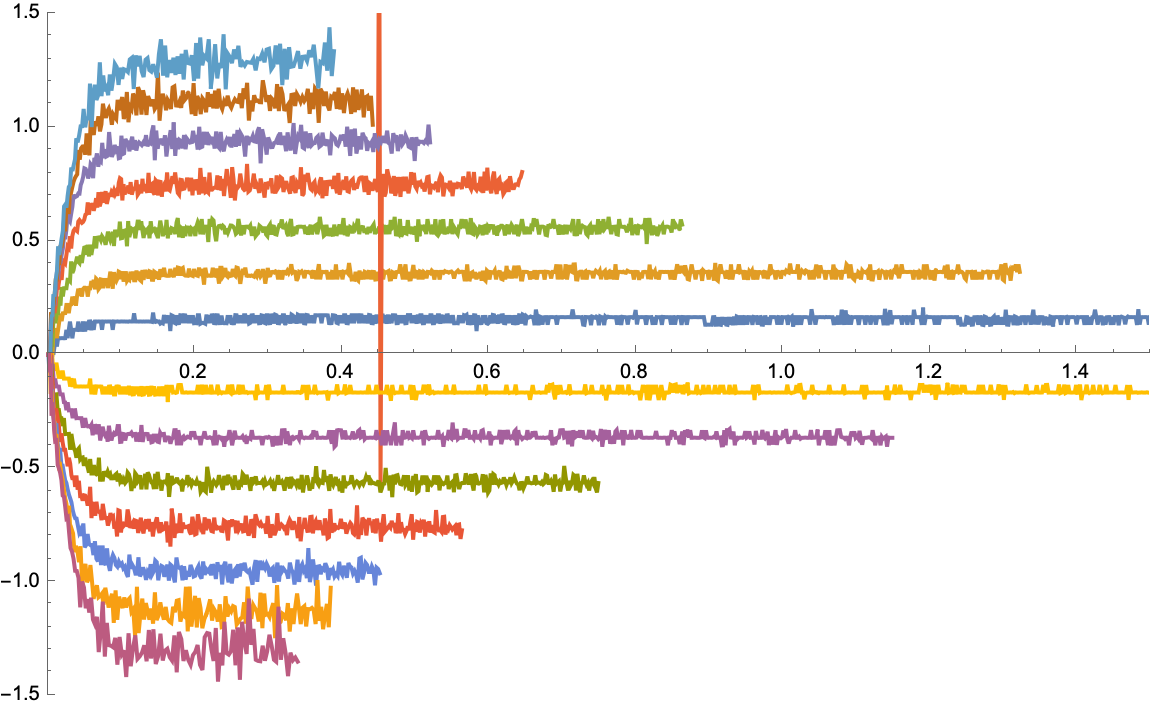
\includegraphics[width=\textwidth]{angular_velocities}
\end{figure}

Mathematica's \texttt{FindFit} function can be used to find the best parameters to fit an expression to a dataset. If we use it to fit our velocity equation to this dataset and plot it on top, it looks like this

\begin{figure}[H]
  \centering
  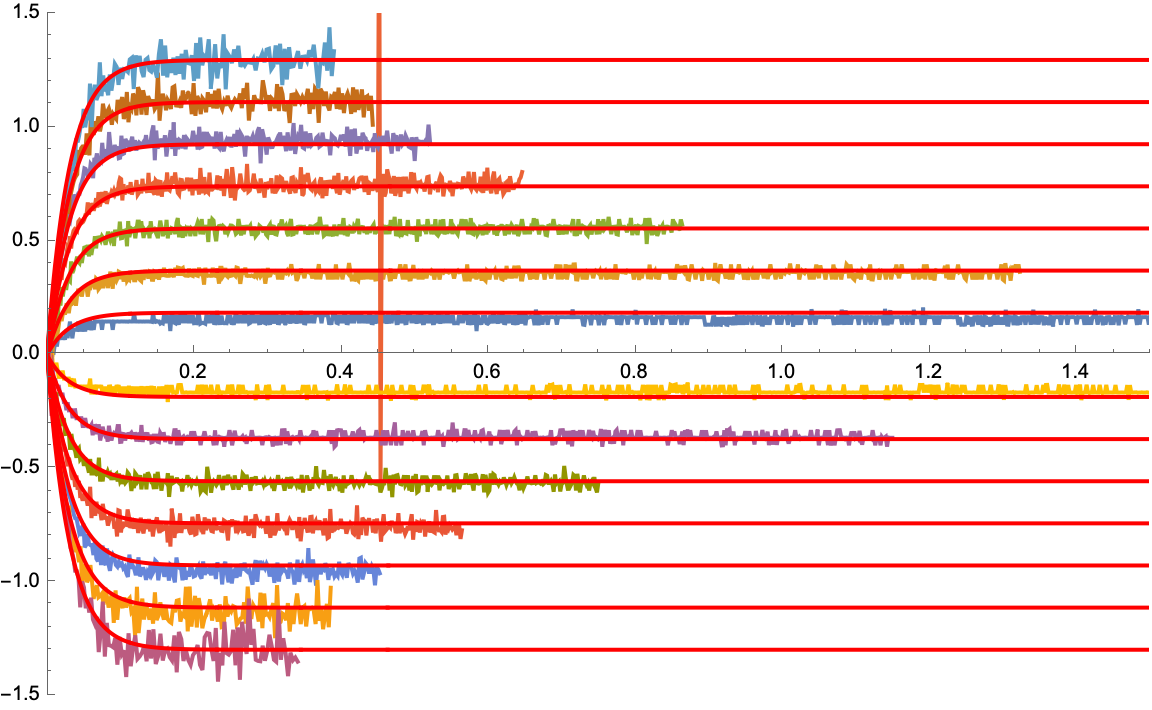
\includegraphics[width=\textwidth]{angular_velocities_fitted}
\end{figure}

A pretty good fit! One last step and we're done.

We have an equation for the cart's velocity over time but it's not very useful. Firstly because it assumes a constant voltage and we're going to be changing the voltage to move the cart back and forth. Secondly, remember, we're trying to find an equation to convert a force into voltage and this equation doesn't involve force at all!

How can we fix this? Newton's second law tells us that $F = m a$. If we can find an equation for the acceleration of the cart based on the input voltage, we could rearrange Newton's second law to get the voltage in terms of the force which is what we're looking for!

Let's take the derivative of our velocity equation with respect to time \[a = d_1 d_2 V_\text{in} e^{-d_2 t}.\] This looks promising, but it still assumes a constant voltage and what value would we use for $t$? Let's keep looking.

Earlier we found a time-indepdendent equation for the angular velocity of the motor \[b_1 \ddot{\omega} + b_2 \dot{\omega} + b_3 \omega + V_\text{in} = 0.\] If we assume that the first term is small and can be ignored \[b_2 \dot{\omega} + b_3 \omega + V_\text{in} = 0,\] multiply by the radius of the timing pulley \[b_2 \dot{v} + b_3 v + R V_\text{in} = 0,\] rearrange, and collect constants we get an equation for the cart's acceleration that doesn't involve time \[\dot{v} = a = k_1 v + k_2 V_\text{in}.\]

We don't know the values of these constants $k_1$ and $k_2$ but we can find them if we equate this equation with our other one for the cart's acceleration. Doing that we finally get our time-independent equation for the cart's acceleration \[a = d_1 d_2 V_\text{in} - d_2 v.\]

Is this equation correct though? One way to check is to integrate it numerically and see if the result matches the data we collected. Back in the Mathematica notebook we do that, and can see it matches pretty well.

Finally we can multiply the cart's acceleration by its mass to find the applied force \[F = m_2 (d_1 d_2 V_\text{in} - d_2 v)\] and we can rearrange that equation to find the voltage required to apply that force \[V_\text{in} = \frac{1}{d_1} \left( v + \frac{F}{d_2 m_2} \right).\] So the control algorithm tells us what force to apply and this equation tells us what voltage to apply. We're ready to start coding!

\section{Code}

This is the code that runs the system. One of its most important jobs is to observe signals from the rotary encoders so we know the motor and pendulum angles. That's achieved with these two interrupt handlers. They're called when the signal from a rotary encoder changes, they calculate the angle change, and update the appropriate variable.

The rest of the system is a big state machine. It moves through a series of initialisation states, starts running, and finally gets killed for one reason or another.

On startup we don't know the position of the cart, so in the first state the cart moves to the right until it's pressing the limit switch. At that point we know where the cart is which lets us zero the cart position and motor angle.

Next, the cart moves to the middle of the track which is where we want it to be when it starts running.

We also need to zero the pendulum angle. The pendulum might still be swinging from the cart's movement, so we wait until it's still, assume it's pointing down, and zero it. This does mean that down is considered zero instead of up, but that's fixed in the next state.

The user rotates the pendulum until it's near upright, we offset the pendulum angle so up is consdered zero, and we start running.

If the cart gets too close to either end of the track or the pendulum angle becomes too great, we assume we're not going to be able to recover, and kill the system. You can also kill it manually by pressing the limit switch.

The last significant part of the code is calculating the cart's velocity and the pendulum's angular velocity. On each iteration of the main loop we record the cart's position, the pendulum's angle, and the time. We store the last $10$ of these values and calculate the velocities as the difference between the most recent value and the oldest value, divided by the difference in their times. I was originally using lower resolution rotary encoders and this method didn't work very well. I tried more complicated numerical differentiation approaches but they were all quite slow. Upgrading to higher resolution rotary encoders let me use this faster and simpler method.

\section{Conclusion}

And that's how I built my self-balancing pendulum!

The 3D models, code, notes, and everything else are available on GitHub which I've linked in the description.

I hope you enjoyed the video, please let me know if you have any feedback or questions. Thanks for watching!

\end{document}